% ******************************* PhD Thesis Template **************************
% Please have a look at the README.md file for info on how to use the template

\documentclass[a4paper,12pt,times,numbered,print,index,openany]{Classes/PhDThesisPSnPDF}
\linespread{1.5}
% ******************************************************************************
% ******************************* Class Options ********************************
% *********************** See README for more details **************************
% ******************************************************************************

% `a4paper'(The University of Cambridge PhD thesis guidelines recommends a page
% size a4 - default option) or `a5paper': A5 Paper size is also allowed as per
% the Cambridge University Engineering Deparment guidelines for PhD thesis
%
% `11pt' or `12pt'(default): Font Size 10pt is NOT recommended by the University
% guidelines
%
% `oneside' or `twoside'(default): Printing double side (twoside) or single
% side.
%
% `print': Use `print' for print version with appropriate margins and page
% layout. Leaving the options field blank will activate Online version.
%
% `index': For index at the end of the thesis
%
% `draft': For draft mode without loading any images (same as draft in book)
%
% `draftmode': Special draft mode with line numbers, images, and water mark with
% timestamp and custom text. Position of the text can also be modified.
%
% `abstract': To generate only the title page and abstract page with
% dissertation title and name, to submit to the Student Registry
%
% `chapter`: This option enables only the specified chapter and it's references
%  Useful for review and corrections.
%
% ************************* Custom Page Margins ********************************
%
% `custommargin`: Use `custommargin' in options to activate custom page margins,
% which can be defined in the preamble.tex. Custom margin will override
% print/online margin setup.
%
% *********************** Choosing the Fonts in Class Options ******************
%
% `times' : Times font with math support. (The Cambridge University guidelines
% recommend using times)
%
% `fourier': Utopia Font with Fourier Math font (Font has to be installed)
%            It's a free font.
%
% `customfont': Use `customfont' option in the document class and load the
% package in the preamble.tex
%
% default or leave empty: `Latin Modern' font will be loaded.
%
% ********************** Choosing the Bibliography style ***********************
%
% `authoryear': For author-year citation eg., Krishna (2013)
%
% `numbered': (Default Option) For numbered and sorted citation e.g., [1,5,2]
%
% `custombib': Define your own bibliography style in the `preamble.tex' file.
%              `\RequirePackage[square, sort, numbers, authoryear]{natbib}'.
%              This can be also used to load biblatex instead of natbib
%              (See Preamble)
%
% **************************** Choosing the Page Style *************************
%
% `default (leave empty)': For Page Numbers in Header (Left Even, Right Odd) and
% Chapter Name in Header (Right Even) and Section Name (Left Odd). Blank Footer.
%
% `PageStyleI': Chapter Name next & Page Number on Even Side (Left Even).
% Section Name & Page Number in Header on Odd Side (Right Odd). Footer is empty.
%
% `PageStyleII': Chapter Name on Even Side (Left Even) in Header. Section Number
% and Section Name in Header on Odd Side (Right Odd). Page numbering in footer


% ********************************** Preamble **********************************
% Preamble: Contains packages and user-defined commands and settings
% ******************************************************************************
% ****************************** Custom Margin *********************************

% Add `custommargin' in the document class options to use this section
% Set {innerside margin / outerside margin / topmargin / bottom margin}  and
% other page dimensions
\ifsetCustomMargin
  \RequirePackage[left=37mm,right=30mm,top=35mm,bottom=30mm]{geometry}
  \setFancyHdr % To apply fancy header after geometry package is loaded
\fi

% *****************************************************************************
% ******************* Fonts (like different typewriter fonts etc.)*************

% Add `customfont' in the document class option to use this section

\ifsetCustomFont
  % Set your custom font here and use `customfont' in options. Leave empty to
  % load computer modern font (default LaTeX font).
  \RequirePackage{helvet}
\fi

% *****************************************************************************
% **************************** Custom Packages ********************************

% ************************* Algorithms and Pseudocode **************************

%\usepackage{algpseudocode}


% ********************Captions and Hyperreferencing / URL **********************

% Captions: This makes captions of figures use a boldfaced small font.
%\RequirePackage[small,bf]{caption}

\RequirePackage[labelsep=space,tableposition=top]{caption}
\renewcommand{\figurename}{Fig.} %to support older versions of captions.sty


% *************************** Graphics and figures *****************************

%\usepackage{rotating}
%\usepackage{wrapfig}

% Uncomment the following two lines to force Latex to place the figure.
% Use [H] when including graphics. Note 'H' instead of 'h'
%\usepackage{float}
%\restylefloat{figure}

% Subcaption package is also available in the sty folder you can use that by
% uncommenting the following line
% This is for people stuck with older versions of texlive
%\usepackage{sty/caption/subcaption}
\usepackage{subcaption}

% ********************************** Tables ************************************
\usepackage{booktabs} % For professional looking tables
\usepackage{multirow}

%\usepackage{multicol}
%\usepackage{longtable}
%\usepackage{tabularx}


% ***************************** Math and SI Units ******************************

\usepackage{amsfonts}
\usepackage{amsmath}
\usepackage{amssymb}
\usepackage{siunitx} % use this package module for SI units


% ******************************* Line Spacing *********************************

% Choose linespacing as appropriate. Default is one-half line spacing as per the
% University guidelines

% \doublespacing
% \onehalfspacing
% \singlespacing


% ************************ Formatting / Footnote *******************************

% Don't break enumeration (etc.) across pages in an ugly manner (default 10000)
%\clubpenalty=500
%\widowpenalty=500

%\usepackage[perpage]{footmisc} %Range of footnote options


% *****************************************************************************
% *************************** Bibliography  and References ********************

%\usepackage{cleveref} %Referencing without need to explicitly state fig /table

% Add `custombib' in the document class option to use this section
\ifuseCustomBib
   \RequirePackage[square, sort, numbers, authoryear]{natbib} % CustomBib

% If you would like to use biblatex for your reference management, as opposed to the default `natbibpackage` pass the option `custombib` in the document class. Comment out the previous line to make sure you don't load the natbib package. Uncomment the following lines and specify the location of references.bib file

%\RequirePackage[backend=biber, style=numeric-comp, citestyle=numeric, sorting=nty, natbib=true]{biblatex}
%\bibliography{References/references} %Location of references.bib only for biblatex

\fi

% changes the default name `Bibliography` -> `References'
\renewcommand{\bibname}{References}


% *****************************************************************************
% *************** Changing the Visual Style of Chapter Headings ***************
% This section on visual style is from https://github.com/cambridge/thesis

% Uncomment the section below. Requires titlesec package.

%\RequirePackage{titlesec}
%\newcommand{\PreContentTitleFormat}{\titleformat{\chapter}[display]{\scshape\Large}
%{\Large\filleft{\chaptertitlename} \Huge\thechapter}
%{1ex}{}
%[\vspace{1ex}\titlerule]}
%\newcommand{\ContentTitleFormat}{\titleformat{\chapter}[display]{\scshape\huge}
%{\Large\filleft{\chaptertitlename} \Huge\thechapter}{1ex}
%{\titlerule\vspace{1ex}\filright}
%[\vspace{1ex}\titlerule]}
%\newcommand{\PostContentTitleFormat}{\PreContentTitleFormat}
%\PreContentTitleFormat


% ******************************************************************************
% ************************* User Defined Commands ******************************
% ******************************************************************************

% *********** To change the name of Table of Contents / LOF and LOT ************

%\renewcommand{\contentsname}{My Table of Contents}
%\renewcommand{\listfigurename}{My List of Figures}
%\renewcommand{\listtablename}{My List of Tables}


% ********************** TOC depth and numbering depth *************************

\setcounter{secnumdepth}{2}
\setcounter{tocdepth}{2}


% ******************************* Nomenclature *********************************

% To change the name of the Nomenclature section, uncomment the following line

%\renewcommand{\nomname}{Symbols}


% ********************************* Appendix ***********************************

% The default value of both \appendixtocname and \appendixpagename is `Appendices'. These names can all be changed via:

%\renewcommand{\appendixtocname}{List of appendices}
%\renewcommand{\appendixname}{Appndx}

% ******************************** Draft Mode **********************************

% Uncomment to disable figures in `draftmode'
%\setkeys{Gin}{draft=true}  % set draft to false to enable figures in `draft'

% These options are active only during the draft mode
% Default text is "Draft"
%\SetDraftText{DRAFT}

% Default Watermark location is top. Location (top/bottom)
%\SetDraftWMPosition{bottom}

% Draft Version - default is v1.0
%\SetDraftVersion{v1.1}

% Draft Text grayscale value (should be between 0-black and 1-white)
% Default value is 0.75
%\SetDraftGrayScale{0.8}


%% Todo notes functionality
%% Uncomment the following lines to have todonotes.

%\ifsetDraft
%	\usepackage[colorinlistoftodos]{todonotes}
%	\newcommand{\mynote}[1]{\todo[author=kks32,size=\small,inline,color=green!40]{#1}}
%\else
%	\newcommand{\mynote}[1]{}
%	\newcommand{\listoftodos}{}
%\fi

% Example todo: \mynote{Hey! I have a note}




% ************************ Thesis Information & Meta-data **********************
% Thesis title and author information, refernce file for biblatex
% ************************ Thesis Information & Meta-data **********************
%% The title of the thesis
\title{New LSB-pair methods to reduce distortion of watermarked image}
%\texorpdfstring is used for PDF metadata. Usage:
%\texorpdfstring{LaTeX_Version}{PDF Version (non-latex)} eg.,
%\texorpdfstring{$sigma$}{sigma}

%% Subtitle (Optional)
\subtitle{COMP90055 \space \space \space 25 points}

%% The full name of the author
\author{Shuyan Hu}



%% Department (eg. Department of Engineering, Maths, Physics)
\dept{874083}

%% University and Crest
\university{University of Melbourne\\
 \\ 
Supervisor: Udaya Parampalli}
\crest{
\includegraphics[width=0.35\textwidth]{image/unimelb.png}}

%% You can redefine the submission text:
% Default as per the University guidelines:
% ``This dissertation is submitted for the degree of''
%\renewcommand{\submissiontext}{change the default text here if needed}

%% Full title of the Degree
\degree{Master of Information Technology}

%% College affiliation (optional)
\college{School of Engineering\\
Conventional Research Project}

%% Submission date
% Default is set as {\monthname[\the\month]\space\the\year}
%\degreedate{September 2014} 

%% Meta information
% \subject{LaTeX} \keywords{{LaTeX} {PhD Thesis} {Engineering} {University of
% Cambridge}}
\subject{874083}


% ***************************** Abstract Separate ******************************
% To printout only the titlepage and the abstract with the PhD title and the
% author name for submission to the Student Registry, use the `abstract' option in
% the document class.

\ifdefineAbstract
 \pagestyle{empty}
 \includeonly{Declaration/declaration, Abstract/abstract}
\fi

% ***************************** Chapter Mode ***********************************
% The chapter mode allows user to only print particular chapters with references
% Title, Contents, Frontmatter are disabled by default
% Useful option to review a particular chapter or to send it to supervisior.
% To use choose `chapter' option in the document class

% \ifdefineChapter
%  \includeonly{Chapter3/chapter3}
% \fi

% ******************************** Front Matter ********************************
\begin{document}

\frontmatter

\begin{titlepage}
  \maketitle
\end{titlepage}


%% ******************************* Thesis Dedidcation ********************************

\begin{dedication} 

This dissertation is dedicated to my supervisor Udaya Parampalli who showed me the charming of doing research.

\end{dedication}


% ******************************* Thesis Declaration ********************************

\begin{declaration}

I certify that\\

This thesis does not incorporate without acknowledgement any material previously submitted for a degree or diploma in any university; and that to the best of my knowledge and belief it does not contain any material previously published or written by another person where due reference is not made in the text. The thesis is 6710 words in length (excluding text in images, table, bibliographies and appendices).

% - where necessary I have received clearance for this research from the University's Ethics Committee
% (Approval Number ....) and have submitted all required data to the Department\\



% Author and date will be inserted automatically from thesis.tex \author \degreedate

\end{declaration}


% ************************** Thesis Acknowledgements *****************************

\begin{acknowledgements}      

First and foremost, I would like to express my sincere gratitude to my supervisor, Associate Professor and Reader Udaya Parampalli. Who leaded me to start doing research step by step. He is a wise man and always a source of knowledge. His attentive mentoring is the primary support that makes this thesis possible.

I would like to thank Patrick Vicky and Peter Uchenna Eze who are the Ph.D. students of Associate Professor Udaya. They helped me in choosing my research topic and correcting me from mistakes when doing research. Besides, Patrick Vicky did proof reading for this thesis; helped me fix grammar mistakes and gave me suggestions to improve the quality of this thesis.

In addition, I would give a thank you to Winnie Nie, my sincere friend. Who provided grayscale images for me. She is always be there by my side during my most hard time and her persistent encourages helps me to fight towards my goals. Without her earnest help, this thesis would not have been possible.

I acknowledge Fangming, who I never met him before. He laid the foundation theories of the LSB-pair method. This thesis is developed and modified based on his theory. 

I would like to express me deep appreciation to my friend, Long Chen who gave me suggestions to improve my codes and helped me optimise the algorithm complexity. I would also like to thanks Larry Zhang, Henry Liu, Joseph Zhang, Sunny Song and Darkspede technical team. With their help in both academic research and real life, I firmed my confidence to finish this thesis. 

Also a thank you to my parents, for their unconditional love, and encouragement also for their financial assistance that supported me to finish this thesis. 

\end{acknowledgements}

% ************************** Thesis Abstract *****************************
% Use `abstract' as an option in the document class to print only the titlepage and the abstract.
\begin{abstract}
Digital watermarking is a technology which can hide security messages into digital image, video and audio. On images, a common method for digital watermarking is done by using the Least Significant Bit (LSB) of pixels as carrier to embed the secret message. However, this modification may disturb carrier image pixel distribution and thus introduces distortion, which increases the likelihood of being detected. This thesis proposes a new method named LSB-pair and its extension methods to reduce watermarked image distortion. These methods are based on LSB replacement; hence, they can be considered as variations of LSB replacement. In evaluating these methods, we set up experiments with 10,000 images as cover data written in MATLAB.  Three image quality measurements are used to evaluate the resulting images: peak signal-to-noise ratio (PSNR), structural similarity index measure (SSIM) and histogram absolute error (Hae). The results displayed the characteristics of each method -- compared with original LSB method, after embedding message, the proposed methods have 28.3\% lower distortion on average but have worse performance on SSIM. Extensive experimentation shows that these new methods are reliable and provide stable performance in reducing watermarked image distortion.
\end{abstract}


% *********************** Adding TOC and List of Figures ***********************

\tableofcontents
\listoffigures
\listoftables

% \printnomencl[space] space can be set as 2em between symbol and description
%\printnomencl[3em]

% \printnomencl

% ******************************** Main Matter *********************************
\mainmatter

%*******************************************************************************
%*********************************** First Chapter *****************************
%*******************************************************************************

\chapter{Introduction}  %Title of the First Chapter

\ifpdf
    \graphicspath{image/}
\fi


%********************************** %First Section  **************************************
%\section{\label{sec:level1}Introduction}

With the fast development of communication technologies, information security has become an important topic. The ease of sharing of multimedia files such as images, videos and text leads to the need of strong copyright protection. Steganography is the study of writing information in the background, with the aim of transmitting information in an undetectable way. Digital watermarking is a part of steganography, it is a technical approach to hide information into digital media. This technology can be used for anonymous payment and digital signature as well as vote, enhance WSN network, protect the copyright and control digital files copy times. Digital watermarking is supposed to be imperceptible ~\cite{chen2001quantization} so that we need to ensure human’s visual system cannot find the difference between original image and watermarked image ~\cite{ker2004improved}. 

The Least-Significant-Bit (LSB) is one of the most common and simple methods in digital watermarking. It embeds message bits into the carrier image pixel's last bits if the message length is less than the carrier image contains pixels ~\cite{ker2004improved}~\cite{kaur2013image}. When a message is embedded into an image, it is unavoidable that the original image changes as a result. The unusual image pixel changes will increase the risk of watermarked images been detected by malicious users. It also means risking the secured information disclosure. 

Aiming to better hide information and increase the security, there is a demand to improve original LSB replacement method by reducing distortion of watermarked images. Jessica Fridrich  \textit{et al} ~\cite{fridrich2003higher} put forward a new watermarking image detection method called pair analysis. From this inspiration, we propose a new method using the pair analysis idea which aims to reduce the distortion of the watermarked image. This method, named LSB-pair, is considered as an advanced LSB replacement method. It can also be regarded as a modification of adaptive pixel pair matching (PPM) which Wien Hong had introduced in 2012 ~\cite{hong2012novel}.  However, the improvement of LSB-pair is not significant comparing with original LSB method. This paper discusses a series of extension LSB-pair methods to improve the performance of LSB-pair.

The rest of this thesis is organized as follows. Chapter 2 briefly reviews existing work in LSB and pair analysis. LSB-pair method and three advanced LSB-pair methods are introduced in Chapter 3. Chapter 4 utilizes three image quality measurement approaches to evaluate these methods and compare their performance. Finally, the conclusion and future work is drawn in Chapter 5.

%*******************************************************************************
%****************************** Second Chapter *********************************
%*******************************************************************************

\chapter{Existing work}

\ifpdf
    \graphicspath{image/}
\fi


% \section{\label{sec:level1}Existing work}

One of the earliest study on digital image watermarking technology was conducted by Tirkel ~\cite{tirkel1993electronic}. He proposes two methods to hide information, both based on changing the carrier image pixel value of Least Significant Bit (LSB). Preceding this paper was a study by Kurah and McHughes, who put forward the idea of \textit{image downgrading} to embed the information into the last bit of pixel in 1992 ~\cite{kurak1992cautionary}. 

Abdullah Bamatraf \textit{et al.} in their paper “A New Digital Watermarking Algorithm Using Combination of Least Significant Bit (LSB) and Inverse Bit” proposes a new LSB method. This method can provide better Peak Signal-to-Noise Ratio (PSNR) value by inverting embed message bits and shifting the order of carrier image pixels ~\cite{bamatraf2011new}. Jessica J Fridrich \textit{et al.} point out the similar idea that the imbalanced distribution of embedding distortion is vulnerable to steganalysis ~\cite{fridrich2001detecting}.

Andrew Ker in his paper “Steganography using multiple-base notational system and human vision sensitivity” points out that the original digital watermarking LSB replacement existing an imbalance of embedding distortion when embedding message into the image. Due to the existence of this imbalance, the LSB can be easily detected ~\cite{ker2004improved}. 

In 2006, Jarno Mielikainen in his paper “LSB matching revisited” mentioned a new embedding algorithm to find a pair of pixels. In his algorithm, two pixels are grouped as a unit, and LSB embedding is done per unit. When storing the same amount of information, this method results in less distortion to the cover image. He also shows that the resistance of watermarking detection can be increased, with the help of reducing image distortion ~\cite{mielikainen2006lsb}. Xinpeng Zhang et al improved Mielikainen’s methods by using exploiting modification direction (EMD) in the same year ~\cite{zhang2006efficient}.

Wien Hong \textit{et al.} in their paper proposes a new method based on pixel pair matching (PPM). This method uses the value of pixels to find a pair pixel in its neighbourhood according to the embedded message bit. His adaptive pixel pair matching (APPM) method offers lower distortion than optimal pixel adjustment process (OPAP) and regular PPM methods for various payloads ~\cite{hong2012novel}.

%*******************************************************************************
%****************************** Third Chapter *********************************
%*******************************************************************************

\chapter{Proposed Methods}

\ifpdf
    \graphicspath{image/}
\fi


% \section{\label{sec:level1}Proposed Methods}

In this part, a new LSB replacement method named LSB-pair which is based on pair pixel matching is proposed. Some extension LSB-pair methods have been developed from this idea, extending its application range. In this part, all methods are designed to embed messages into grayscale image, where pixel values are stored as 8 bit unsigned integers. In order to differentiate the existing LSB replacement method and our modified LSB methods; we use \textit{original LSB replacement method} or \textit{regular LSB replacement method} to represent the \textit{existing LSB replacement method}; we use \textit{extension LSB-pair methods} to indicate our extension methods which based on LSB-pair method; we use \textit{the LSB-pair methods} to represent LSB-pair and its extension methods.


\section{\label{sec:level1}LSB-pair}

This function, named LSB-pair, tries to find pairs of pixels which would reduce watermarked image distortion from embedding. Before the start of pair detection, the carrier image should be transformed into a one-dimensional data. Figure 3.1 shows how to convert a picture, which is two-dimensional, into one dimension.

\begin{figure}[H]
 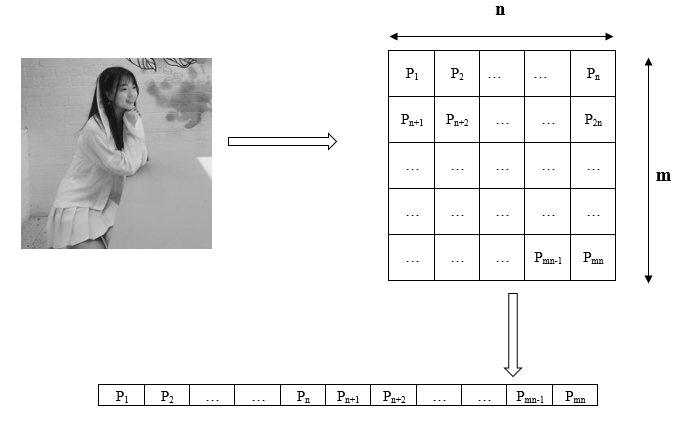
\includegraphics[width=\columnwidth]{image/Convert_image_as_one-dimension_matrix.png}
 \caption{Convert image as one-dimension matrix}
 \label{fig:figure}
\end{figure}

With one-dimension data structure, we can use an array list to denote any pixels in the carrier image. For instance, \(P_{i}\) represents a specific pixel in the carrier image, with \(i\) denoting its sequence number in the data. Symbol \(G(P_{i})\) means the value of gray level in pixel \(P_{i}\). The value of \(G(P_{i})\) is an integer which ranges from 0 to 255. When converting watermarked message into binary, we can use \(M_{i}\) to present the \(i^{th}\) binary value of this watermarking message. Hence, the value of \(M_{i}\) is either 0 or 1. \(M_{i}\) and \(M_{i+1}\) are corresponding message bits respectively for \(P_{i} \text{ and } P_{i+1}\). Finally, the notation \(LSB(G(P_{i}))\) represents the last bit of gray level value on this pixel. For example, if the gray level of the \(28^{th}\) pixel was 125, we could use math formula \(LSB(G(P_{28})) = 1\) to present the LSB of \(28^{th}\) pixel. If the gray level of the \(29^{th}\) pixel was 126, we had \(LSB(G(P_{29}))\) is 0, etc. 

Based on the definition above, two adjacent pixels \(P_{i}\) and \(P_{i+1}\) are regarded as a LSB-pair pixels if they satisfy the conditions (3.1) and (3.2): 

\begin{equation}
\\ G(P_{i}) = G(P_{i+1}) + 1 \quad \text{ or } \quad G(P_{i}) = G(P_{i+1}) - 1
\end{equation}
\begin{equation}
LSB(G(P_{i})) \neq M_{i} \quad \text{ and } \quad LSB(G(P_{i+1})) \neq M_{i+1}
\end{equation}

We can use one sentence to conclude this definition: \textit{two adjacent pixels with adjacent gray levels and their LSB are different from corresponding message bits}.

After obtaining our LSB pairs, the next step is to find out how the distortion changes when embedding the message. Due to the fact that each pixel in grayscale image occupies 8 bits, we can use a list of 256 ordered elements to represent the image energy distribution or we can call it distortion directly. Each element means the frequency of a specific gray level. The distortion list may be written as:
\[D = (d_{0}, d_{1}, d_{2} … , d_{253}, d_{254}, d_{255})\]
For example, \(d_{35} = 47\) represents the total number of gray level 35 is 47. In order to calculate the distortion changes after watermarking, the original image distortion \(d_{1}\) and the watermarked image distortion \(d_{2}\) are required. The difference between \(d_{1}\) and \(d_{2}\): \(D’ = d_{2} - d_{1}\) is the distortion change which will be used in the latter evaluation. In this case: \(D’ = (d’_{0}, d’_{1}, d’_{2}…, d’_{253}, d’_{254}, d’_{255})\), \(d’35 = 47\) means the frequency of gray level 35 in watermarked image is 47 greater than original image. Therefore, if no message is embedded, all elements in \(D’\) should be 0.


There are two different situations when using LSB-pair method to embed messages. Firstly, suppose there are two pixels: \(G(P_{i}) = 124\), \(G(P_{i+1}) = 125\) and message bits: \(M_{i} = 1\), \(M_{i+1} = 0\). The LSB value of these two pixels can be obtained from calculation: \(LSB(G(P_{i})) = 0\), \(LSB(G(P_{i+1})) = 1\). Because these pixels meet the requirements (3.1) and (3.2), they are regarded as a pair. Assuming the distortion change before doing LSB replacement is:
\[D’_{before} = (…, d_{124} = a, d_{125} = b, …)\]
Then embed the $i^{\text{th}}$ message bit into this image, we have new \(G'(P_{i})\) and \(D’_{after}\): 
\[G’(P_{i}) = 125\]
\[D’_{after} = (…, d_{124} = a - 1, d_{125} = b + 1, …)\]

Then embed the $(i+1)^{\text{th}}$ message bit into this image, we have new \(G’(P_{i+1})\) and \(D’_{after}\): 
\[G’(P_{i+1}) = 124\]
\begin{align*} 
D’_{after}  &= (…, d_{124} = a - 1 + 1, d_{125} = b + 1 - 1, …)\\
            &= (…, d_{124} = a, d_{125} = b, …)\\
            &= D’_{before}
\end{align*}
\[ \Rightarrow D’_{after} - D’_{before} = 0\]
In this situation, distortion difference equals to 0 means that the distortion is not changed after embedding watermarking messages.

Another situation is that when \(G(P_{i}) = 125\), \(G(P_{i+1}) = 126\), \(M_{i} = 0\), \(M_{i+1} = 1\). Assume the distortion change before watermarking is \(D’_{before} = (…, d_{124} = a, d_{125} = b, d_{126} = c, d_{127} = d, …)\). Then using LSB replacement method to embed message, we have: 
\[G’(P_{i}) = 124\] 
\[G’(P_{i+1}) = 127\]
\[D’_{after} = (…, d_{124} = a + 1, d_{125} = b - 1, d_{126} = c - 1, d_{127} = d + 1, …)\]


After that, calculating the distortion difference: 
\[D’_{after} - D’_{before} = (|a + 1| - |a|) + (|b - 1| - |b|) + (|c - 1| - |c|) + (|d + 1| - |d|)\]

According to the definition, \(D’_{after} - D’_{before} < 0\) means that after embedding message, the distortion of the image is reduced and vice versa. Assume \(a > 0, b < 0, c < 0 \quad and \quad d > 0\), then we have:

\begin{align*} 
D’_{after} - D’_{before}    &= & & (|a + 1| - |a|) + (|b - 1| - |b|)\\
                            &  & & + (|c - 1| - |c|) + (|d + 1| - |d|)\\
                            &= & & (a + 1 - a) + (1 - b + b) \\
                            &  & & + (1 - c + c) + (d + 1 - d)\\
                            &= & & 1 + 1+ 1+ 1\\
                            &= & & 4 > 0
\end{align*}

However, when \(a + 1 < 0, b - 1 > 0, c - 1 > 0 \quad and \quad d + 1 < 0\)
\begin{align*} 
D'_{after} - D'_{before}    &= & & (|a + 1| - |a|) + (|b - 1| - |b|)\\
                            &  & & +(|c - 1| - |c|) + (|d + 1| - |d|)\\
                            &= & & ( - 1 - a + a) + (b - 1 - b)\\
                            &  & & + (c - 1 - c) + ( - 1 - d + d)\\
                            &= & & - 1 - 1 - 1 - 1\\
                            &= & & -4 < 0
\end{align*}
Besides these two specific situations, there are various permutations and combinations of the value of a, b, c and d. However, in LSB-pair methods, we are only interested in whether if the value of $D’_{after} - D’_{before}$ is positive or negative.  In other words, in this method there are only two interesting situations: increasing change in distortion or decreasing change. Additionally, the distortion change can be 0 in some situations; in order to reduce the algorithm complexity, we regard the distortion as not changing and distortion increasing as the same class.

In the situation of \(G(P_{i}) = 124\), \(G(P_{i+1}) = 125\), the distortion is not changed. Because after embedding, we have: \(G’(P_{i}) = 125, G’(P_{i+1}) = 124\), the total number of gray level 124 and 125 does not change. It looks like these two pixels swap their position (values). It inspires a solution to handle the second situation. Since \(G(P_{i}) = 125, G(P_{i+1}) = 126, M_{i} = 0, M_{i+1} = 1\), if swap the position of two pixels before embedding, the result will be: \(G’(P_{i}) = 126, G’(P_{i+1}) = 125\). Then, using LSB replacement method, it is obvious that the distortion would not change after embedding. However, when applying regular LSB replacement for the second situation directly, the distortion change can be both positive and negative. Hence, the idea of LSB-pair is swapping pixels before using LSB replacement when the distortion change is positive and using regular LSB replacement when distortion change is negative. One thing we need to clear is that the distortion \(D'\) will not change after swapping two pair pixels because the gray level distribution is not changing.

An example to outline how this method works can be found in the FIG 3.2; if there are two pixels, \(G(P_{i}) = 125, G(P_{i+1}) = 126\), we apply LSB replacement at first, then compare the distortion change. Depending on whether it is positive or negative, we can choose between swapping pixels values before using LSB replacement or to use regular LSB replacement directly. 


One more thing we need to pay attention to is that just swapping pixels value is the same as swapping pixels value when using LSB replacement. This conclusion is not hard to prove. From the LSB pair definition, there have two main classes: \circled{1} \(G(P_{i}) = G(P_{i+1}) + 1\) \textit{or} \circled{2} \(G(P_{i}) = G(P_{i+1}) - 1\) . After swapping pixels value, we have \circled{1} \(G(P’_{i}) = G(P_{i}) - 1, G(P’_{i+1}) = G(P_{i+1}) + 1\) \textit{and} \circled{2} \(G(P’_{i}) = G(P_{i}) + 1, G(P’_{i+1}) = G(P_{i+1}) - 1\) which correspond respectively. Then moving to their corresponding message bits: \(LSB(G(P_{i})) \neq M_{i}\) \textit{and} \(LSB(G(P_{i+1})) \neq M_{i+1}\), it is not hard to get that \(LSB(G(P’_{i})) = M_{i}\) \textit{and} \(LSB(G(P’_{i+1})) = M_{i+1}\). The pixels value will not change after applying LSB replacement method, because the last bit of each pixel is the same as its corresponding message bit. With this knowledge, we can reduce the LSB-pair algorithm complexity by simplifying swapping pixels value and apply LSB replacement to swapping pixels value only. 


\begin{figure}[h]
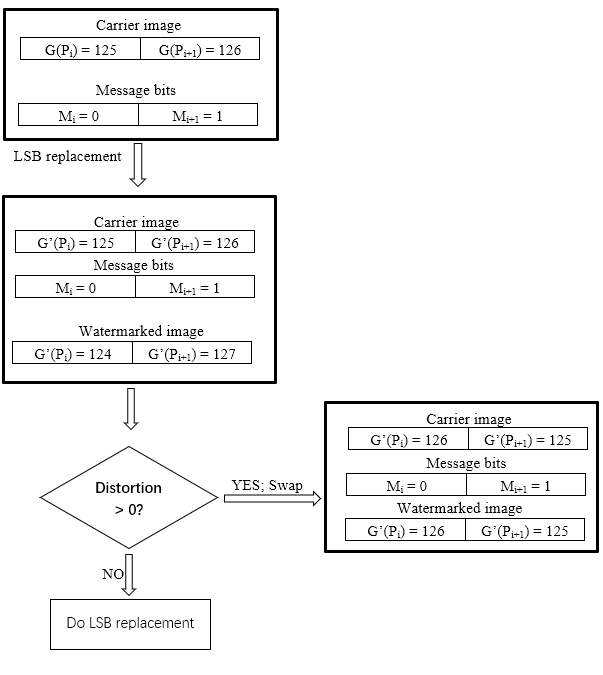
\includegraphics[width=\columnwidth]{image/LSB-pair_example.PNG}
\caption{LSB-pair embedding}
\label{fig:figure}
\end{figure}


In summary, this methods checks each pixel to find out pixel pair which satisfies requirements (3.1) and (3.2). Then we check the distortion change (difference) \(D'_{after} - D'_{before}\); if distortion change is larger than 0, swap two pixels' position. Otherwise, we apply the original LSB replacement method. It can be concluded by following steps (FIG 3.3):
\begin{enumerate}
\item Check current pixel \(P_{i}\) and next pixel \(P_{i+1}\) is a pair or not. If not, go to step (5), otherwise, go to step (2).
\item Calculate the distortion change \(D'_{after} - D_{before}\) for regular LSB replacement, if it larger than 0, go to step (3), otherwise, go to step (4)
\item Swap two pixels position (value), then jump next iteration, go to one after next iteration.
\item Do LSB replacement for this pixel \(P_{i}\) and next pixel \(P_{i+1}\), then jump next iteration, go to one after next iteration.
\item Do LSB replacement for current pixel \(P_{i}\) then go to next iteration for next pixel.
\end{enumerate}




\begin{figure}[h]
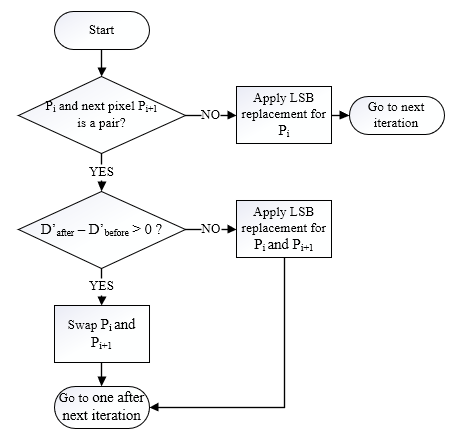
\includegraphics[width=\columnwidth]{image/processing_map.PNG}
\caption{LSB-pair processing map}
\label{fig:figure}
\end{figure}


\section{\label{sec:level1}LSB-triple-pair}

From our experiment for LSB-pair, we found that 0.47\% of pixels meet the requirements (3.1) and (3.2), and 0.25\% of the pixels are in position for swapping to reduce the image distortion. The experiment results show that LSB-pair is rare to find and have very limited performance on reducing watermarked image distortion. With this concern, there is a demand to expand LSB-pair method the range of application. Our modified method called LSB-triple-pair, it changes the requirements of the LSB-pair to expand the range of application.

The LSB-triple-pair method is a modification of LSB-pair which uses three pixels to find a pair. In the previous method, each logic iteration considers two adjacent pixels \(P_{i}\) and \(P_{i+1}\) and their corresponding message bits \(M_{i}\) and \(M_{i+1}\). In this method, three pixels are considered in each iteration: \(P_{i}, P_{i+1} and P_{i+2}\). The idea is, when the first and second pixel do not meet the condition (3.1) and (3.2) or distortion reduce requirements, this algorithm will try to find a pair between the first and third pixel to reduce the image distortion. The processing steps are:

\begin{enumerate}
\item Check current pixel \(P_{i}\) and next pixel \(P_{i+1}\) is a pair or not. If not, go to step (5), otherwise, go to step (2).
\item Calculate the distortion change for regular LSB replacement \(D'_{after} - D_{before}\), if it is \textbf{greater than or equal to} 0, go to step (4), otherwise, go to step (3).
\item Do LSB replacement for this pixel \(P_{i}\) and next pixel \(P_{i+1}\), then go one after next iteration.
\item Check current pixel \(P_{i}\) and the one after next pixel \(P_{i+2}\) is a pair or not. If not, go to step (5), otherwise, go to step (6).
\item Do LSB replacement for pixel \(P_{i}\), \(P_{i+1}\), \(P_{i+2}\) than jump two iterations, go to the fourth iteration.
\item Calculate the distortion change for apply LSB replacement on these three pixels \((D’_{after} - D’_{before})\), if it lager than 0, go to step (7), otherwise, go to step (5).
\item Swap the first and the third pixels position (value), do LSB replacement on the second pixel then jump next two iterations, go to the fourth iteration.
\end{enumerate}

For instance, there are three continuous pixels: \(G(P_{i}) = 125, G(P_{i+1}) = 124, G(P_{i+2}) = 126\), and their corresponding message bits: \(M_{i} = 0, M_{i+1} = 1 M_{i+2} = 1\). In this situation, first two pixels \(P_{i}\) and \(P_{i+1}\) meet the requirements (3.1) and (3.2). However, from the distortion definition, the distortion will not change after applying LSB replacement. Therefore, according to the algorithm, the value of these two pixels will not swap then the process will compare the first pixel with the third pixel. It is clear that \(P_{i}\) and \(P_{i+2}\) meet the requirements (3.1) and (3.2), assuming the distortion change will be greater than 0 after applying regular LSB replacement method, this method will swap \(P_{i}\) and \(P_{i+2}\) value then apply LSB replacement to these three pixels. FIG 3.4 shows the processing map.


\begin{figure}[h]
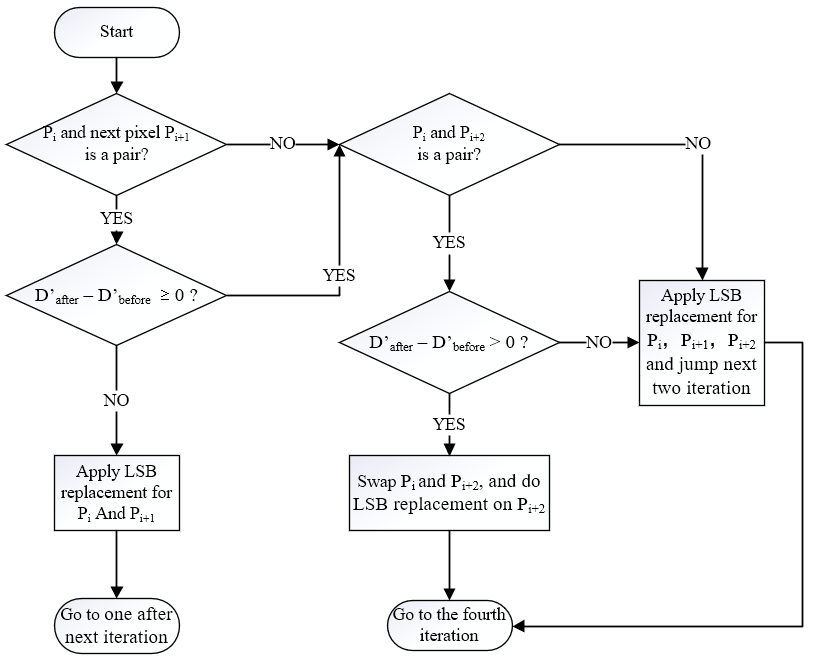
\includegraphics[width=\columnwidth]{image/processing_map_triple.PNG}
\caption{LSB-triple-pair processing map}
\label{fig:figure}
\end{figure}    




\section{\label{sec:level1}LSB-crossLine-pair}

LSB-crossline-pair is another method which extends from LSB-pair. This method tries to find the pixel pairs of current pixel with next line pixel in the carrier image. In this algorithm, we need to change image sequencing from one dimension back to two dimensions. FIG 3.5 shows how this method finds pixel pairs with next line pixel. For example, if the carrier image has \(n\) pixels in horizontal and \(m\) pixels in vertical, this algorithm will try to find a pair between pixel \(P_{i}\) and \(P_{i+n}\). The motivation of this method is also to extend the application range of LSB-pair.  

In this case, in order to avoid embedding system crush, the algorithm will stop LSB-crossline-pair detecting and do LSB-pair detect only when moving to pixel which is in the last row. Another thing that we need to pay attention to is the possibility of jumping to specific iterations. Because the embedding algorithm is from one pixel to next pixel sequentially, for LSB-pair, when a crossline pair is detected, the algorithm would apply original LSB-pair or swap pixels value, then jump two adjacent iterations. However, in LSB-crossline-pair, it cannot jump to the iteration of the next line’s pixel immediately. In code level, it needs an extra list to record the \(P_{i+n}\), if \(P_{i}\) and \(P_{i+n}\) meet all requirements of swapping value. Before each iteration, the code will check this list to see whether we need to jump this iteration or not. However, in fact, this special situation cannot influence the result of LSB-crossline-pair detect. Because if \(P_{i}\) and \(P_{i+n}\) meet the conditions of value swap, the new \(P_{i+n}\) (previous \(P_{i}\)) cannot satisfy requirement (3.2), which is \(LSB(G(P_{i+n})) \neq M_{i+n}\). In our experiments and coding, we skip this swapped pixel checking function, in order to save CPU processing power and memory usage. Furthermore, logically, this makes no sense to check LSB-pair condition for an already swapped value pixel. This can be an optimisation for improving time-consuming and reducing algorithm complexity for LSB-crossline-pair method.  

The processing steps for LSB-crossline-pair are:

\begin{enumerate}
\item Check current pixel \(P_{i}\) is in the jump list or not. If yes, go to next iteration, otherwise, go to step (2).
\item Check current pixel \(P_{i}\) and next pixel \(P_{i+1}\) is a pair or not. If not, go to step (5), otherwise, go to step (3).
\item Calculate the distortion change for using regular LSB replacement \((D’_{after} - D’_{before})\), if it \textbf{greater than or equal to} 0, go to step (5), otherwise, go to step (4)
\item Do LSB replacement for this pixel \(P_{i}\) and next pixel \(P_{i+1}\), then jump next iteration, go to the one after iteration.
\item Check current pixel \(P_{i}\) and the one after next pixel \(P_{i+n}\) is a pair or not. If not, go to step (6), otherwise, go to step (7).
\item Do LSB replacement for pixel \(P_{i}, P_{i+1}, P_{i+n}\) , record \(P_{i+n}\) into jump list then jump next iterations, go to the third iteration.
\item Calculate the distortion change for applying LSB replacement on \(P_{i}\) and \(P_{i+n}\):  \((D’_{after} - D’_{before})\), if it greater than 0, go to step (8), otherwise, go to step (6).
\item Swap \(P_{i}\), and the \(P_{i+n}\) position (value), do LSB replacement on \(P_{i+1}\) then record \(P_{i+n}\) into jump list, after that, jump next iteration, go to the third iteration.
\end{enumerate}

For instance, there are three pixels: \(G(P_{i}) = 125, G(P_{i+1}) = 124, G(P_{i+n}) = 126\), and their corresponding message bits: \(M_{i} = 0, M_{i+1} = 1 M_{i+n} = 1\). In this situation, first two pixels \(P_{i}\) and \(P_{i+1}\) meet the requirements (3.1) and (3.2). However, from the distortion definition, the distortion will not change after applying LSB replacement. Therefore, according to the algorithm, the value of these two pixels will not swap then the process will compare the first pixel \(P_{i}\) with the next line pixel \(P_{i+n}\). It is clear that \(P_{i}\) and \(P_{i+n}\) meet the requirements (3.1) and (3.2), assuming the distortion change will be greater than 0 after applying regular LSB replacement method, this method will swap \(P_{i}\) and \(P_{i+n}\) value then record \(P_{i+n}\) to jump list. After that, apply LSB replacement to these three pixels.

\begin{figure}[h]
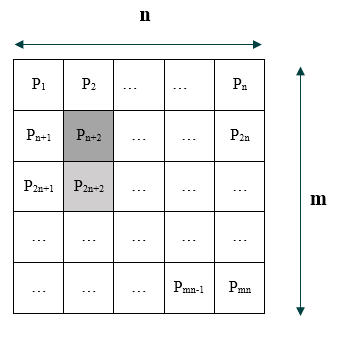
\includegraphics[width=\columnwidth]{image/LSB-crossline-pair.PNG}
\caption{LSB-crossline-pair}
\label{fig:figure}
\end{figure}   




\section{\label{sec:level1}Combination}

This extension method is called LSB-combination-pair; it aims to explore whether the combination of multiple LSB-pair methods can increase the performance of distortion reduction. The series of LSB-pair methods used in this section are LSB-pair, LSB-crossline-pair and LSB-triple-pair. As we have discussed above, all these methods can improve the performance of reducing watermarked image distortion. Therefore, it is possible that combining these three methods into one should have better performance than original LSB replacement as well as any of these three. 

As for the priority of pair finding in LSB-combine-pair. By comparing the performance of LSB-crossline-pair and LSB-triple-pair, the result shows that LSB-crossline-pair have better performance and more consistent in reducing image distortion than LSB-triple-pair. A detailed discussion and analysis of experiment result will be provided in next chapter. Hence, the idea of the new approach is to use LSB pair method at first; if these pixels are not a pair, try to find LSB-crossline-pair. If these pixels still do not meet the requirements of distortion reducing, then try to find a pair using LSB-triple-pair. FIG 3.6 shows a simplification processing map.


\begin{figure}[h]
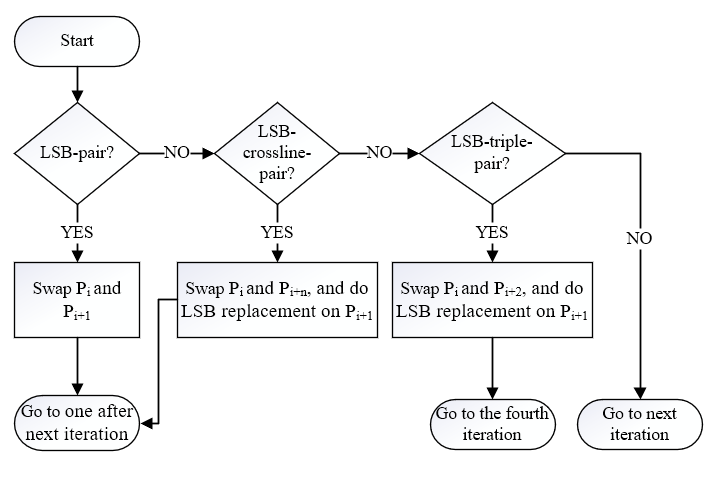
\includegraphics[width=\columnwidth]{image/processing_map_ultra.PNG}
\caption{LSB-combine-pair processing map}
\label{fig:figure}
\end{figure}  
%*******************************************************************************
%****************************** Fourth Chapter *********************************
%*******************************************************************************

\chapter{Evaluation}

\ifpdf
    \graphicspath{image/}
\fi

This section discusses the performance of each LSB-pair methods by using three image quality measurement approaches: Peak signal-to-noise ratio (PSNR), Histogram absolute error (Hae) and Structural similarity index measure (SSIM). In our experiment, we used an image set which came from GHIM-10K  ~\cite{liu2015content} and it contains ten thousand images. In this image set, all images are grayscale images which is either $400 \times 300$ or $300 \times 400$ in resolution. The embedding message is 6,219 English characters in length and encoded with ASCII code standard, 1 byte for each character. We embedded this 6,219 bytes size message into these grayscale images using five LSB embed methods: original LSB replacement, LSB-pair, LSB-crossline-pair, LSB-triple-pair and LSB-combine-pair. 

Before comparing the performance of these methods, one thing that needs to be mentioned is that the error rate of extracting watermarked message by using these methods is 0\% over these 10,000 images. For digital watermarking, the robustness is one of the core requirements. This experiment result shows that these methods are stable and reliable enough to be considered as new methods in digital watermarking field.

\section{\label{sec:level1}Hae}

Histogram absolute error (Hae) is a method which intuitively indicates the total difference between original image and watermarked image. In the previous section we had defined the distortion distribution of gray level pixels is: \(D = (d_{0}, d_{1}, d_{2} … , d_{253}, d_{254}, d_{255})\); the distortion changes between watermarked image and original image is: \(D' = D_{2} - D_{1}, D' = (d'_{0}, d'_{1}, d'_{2} … , d'_{253}, d'_{254}, d'_{255})\). Yang ~\cite{ren2014image} used a formula to calculate histogram absolute error:
$$h(n) = \sum_{i=1}^{H}*\sum_{j=1}^{W}(\delta(n,P(i,j)))$$

where
$$\delta(u,v) = \begin{cases} 1, & u = v \\ 
0, & u \neq v \end{cases}$$

In his formula, H and W is the height and width of the carrier image respectively. P(i,j) is the gray level of a special pixel, in this thesis, it is the same as \(G(P_{i})\) which also refer to the gray level of  pixel \(P_{i}\). The element \textit{n} represents the gray intensity value, for example, in an 8 bits per pixel image, \(n \in [0,255]\) and \(n\in N\). \(255\) comes from \(2^{8} -1\) which is the maximum value of gray level. According to the previous image distortion definition and the image set we used, this formula can be simplified to:

$$h(n) = \sum_{i=1}^{255} d_{i}$$

Then calculate distortion change:
$$Hae = \sum_{i=1}^{255} (d2_{i} - d1_{i}) = \sum_{i=1}^{255} d'_{i}$$

Form the definition, the value of Hae smaller than 0 represents distortion have reduced, vise verse. FIG 4.1 shows the pseudocode of this method.

\begin{figure}[h]
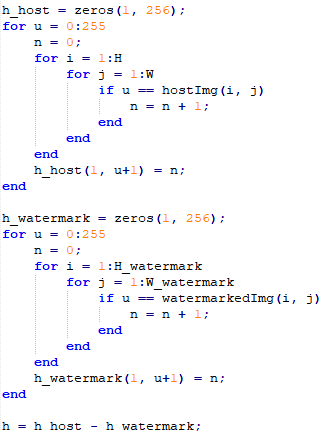
\includegraphics[width=\columnwidth]{image/Pseudocode_Hae.PNG}
\caption{Pseudocode of Hae}
\label{fig:figure}
\end{figure}   



\section{\label{sec:level1}PSNR}

Peak signal-to-noise ratio (PSNR) is one of the most  important and commonly used measurements to evaluate image quality. PSNR is an engineering term for the ratio between the maximum possible power of a signal and the power of corrupting noise that affects the fidelity of its representation. MSE is mean squared error between two images. The higher value of MES represents higher error as well as the worse picture quality ~\cite{eratne2009fast}.

The formula of PSNR is:

\begin{align*}  
PSNR    &=  10* \log_{10} \frac{MAX^2_{1}}{MSE} \\
        &=  20 *\log_{10} \frac{MAX_{1}}{\sqrt{MSE}}
\end{align*} 

which the formula of MSE is:

$$MSE = \frac{1}{mn}\sum_{i=0}^{m-1}\sum_{j=0}^{n-1} [I(i,j)-K(i,j)]^2$$

In PSNR formula, the MAX means the maximum possible value of the image. For example, if there is a picture which is 8 bits per pixel, the maximum value is 255, if it is14 bits, the MAX in this situation is 16383. As for a colourful picture, there has three MSE values corresponding to Red, Green and Blue, and there have three PSNR values for each colour as well. Which means, a colourful image has a vector of three PSNR values to evaluate its quality.


Generally, for PSNR, 30 to 50 dB noise for 8 bits picture, 60 to 80 dB noise for 16bits picture are considered as an acceptable image quality changes. However, PSNR is not friendly for human vision. The value of PSNR is not exactly how we humans think. Because it just uses mean square value to evaluate image, does not consider the image inside, which means, it does not care about what this image is, just evaluate the total and average value or energy changes of these two images.

However, this image quality measurement does not take into account how human's visual system perceives images, which itself may be different for different individuals. It is very complex and cannot be treated as a linear system; the result of human vision evaluation can be influenced by individual’s background, knowledge and motivation. The observation environment is also a significant parameter ~\cite{Tong2006IamgeQuality}. Tong ~\cite{Tong2006IamgeQuality} used FIG 4.2 as an example in his paper. The image in middle is the original image, it is obvious that most people think the left one is more similar than the right one. However, these two have the same PSNR value. For this reason, our experiment only uses PSNR as a reference measurement approach, instead of treating it as a core indicator for image changes.

\begin{figure}[h]
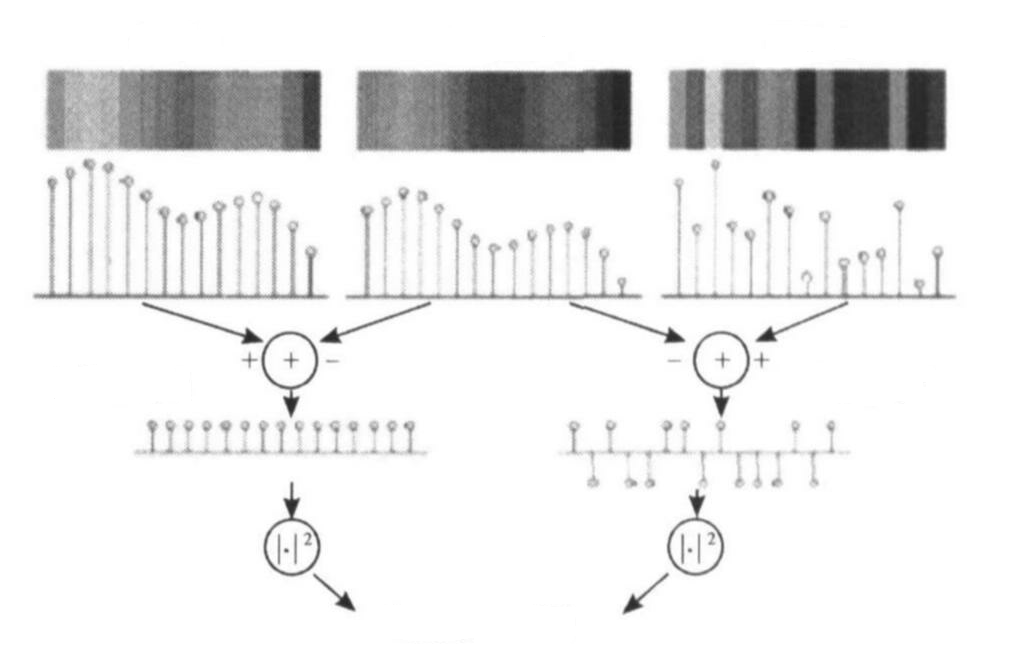
\includegraphics[width=\columnwidth]{image/PSNR_example.png}
\caption{PSNR example \cite{Tong2006IamgeQuality}}
\label{fig:figure}
\end{figure} 


\section{\label{sec:level1}SSIM}

Structural similarity index measure (SSIM) performs well for static image measure. Regular approaches are going to solve absolute errors, however, SSIM is perception-based model which can consider image degradation. Image degradation is considered as a perceived change in the structural information of the image.  It not only considers the RGB (Red, Blue, Green) colour channels, but also YUV (Luminance, Chrominance, Chroma). This approach believes each pixel have strong inter-dependencies especially when they are spatially close.

According to Wang’s research, SSIM has better performance than PSNR but it requires more computing power and processing time to measurement two images. However, it does not totally solve the weaknesses of PSNR. ~\cite{wang2005structural} The algorithm for SSIM is complex, generally, it separates image to various windows and measure between windows. The formula is:

\begin{equation}
SSIM ( f ,g ) = l ( f ,g )c ( f ,g )s ( f ,g )
\end{equation}

\begin{equation}
\begin{cases} l(f,g) = \frac{2\mu_{f}\mu_{g} + C_{1}}{\mu^2_{f} + \mu^2_{g} + C_{1}}\\ 
c(f,g) = \frac{2\sigma_{f}\sigma_{g} + C_{2}}{\sigma^2_{f} + \sigma^2_{g} + C_{2}}\\
s(f,g) = \frac{\sigma_{fg} + C_{3}}{\sigma_{f}\sigma_{g} + C_{3}}
\end{cases}
\end{equation}


The first term in (4.2) is the luminance comparison function which measures the closeness of the two images’ mean luminance \((\mu_{f}\)  and \(\mu_{g})\). c(f,g) is the function of measure contrast comparison, and the third item is for the structure comparison. \(C_{1}\), \(C_{2}\) and \(C_{3}\) is positive constants which are used to provide from null denominator.


\section{\label{sec:level1}Experiment and results}

This section discusses the results of original LSB replacement and four LSB-pair methods using three image quality measurement approaches mentioned in the previous sections. This section goes through one image quality measurement approach by another and compares each LSB method to confirm which method have the best performance for this metric.  

As outlined in the methodology, experiments were done in MATLAB. One grayscale image produces one output image for each of the LSB methods. After embedding messages, the code compares the output images with their original images, then we generate an excel document to display the result.

FIG 4.3 shows the digital watermarked image which is embedded with information invisibly, (a) is the original $512 \times 512$ carrier image. Image (b), (c), (d), (e), (f) are done by original LSB replacement, LSB-pair, LSB-crossline-pair, LSB-triple-pair, LSB-combine-pair respectively. 


% \begin{figure}[h]
% 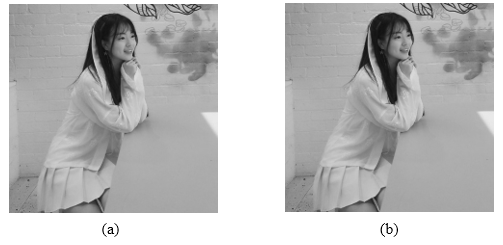
\includegraphics[width=\columnwidth]{image/ab.PNG}
% \label{fig:figure}
% \end{figure} 

% \begin{figure}[h]
% 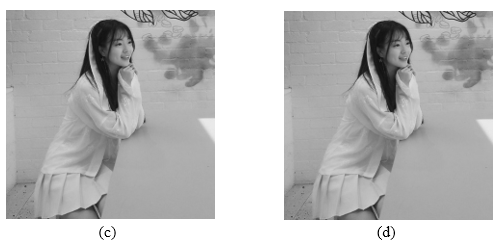
\includegraphics[width=\columnwidth]{image/cd.PNG}
% \label{fig:figure}
% \end{figure} 

% \begin{figure}[h]
% 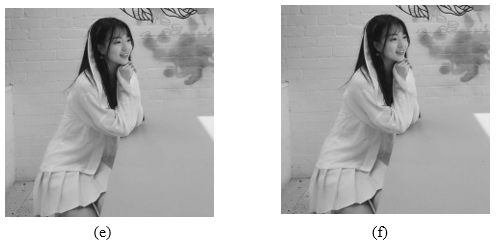
\includegraphics[width=\columnwidth]{image/ef.PNG}
% \caption{Watermarking embedding}
% \label{fig:figure}
% \end{figure} 

\begin{figure}[h]
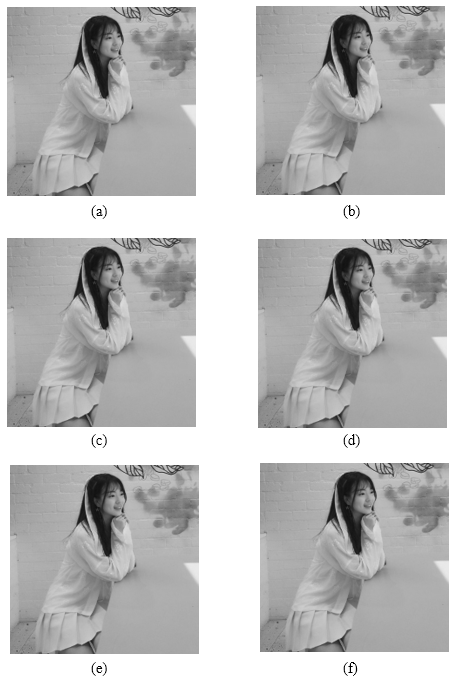
\includegraphics[width=\columnwidth]{image/abcdef.PNG}
\caption{Watermarking embedding}
\label{fig:figure}
\end{figure} 


FIG 4.4 and Table 4.1 show the PSNR results for the regular LSB replacement, LSB-pair, LSB-crossline-pair, LSB-triple-pair and LSB-combine-pair. From the table, it is clear that all these methods have the same PSNR value. These results are the same as our expectation. According to these LSB-pair methods embedding mechanism, it is not hard to prove they have same PSNR value. Here is a prove of original LSB replacement and LSB-pair having same PSNR value: 

\begin{itemize}
  \item If two adjacent pixels are not a pair, they need to be applied for original LSB replacement, hence, the PSNR not change when two pixels are not a pair.
  \item Assuming \(P_{i}, P_{i+1}\) meets LSB pair requirements, \(P_{i} = P_{i+1} + 1\) and \(LSB(P_{i}) = 0\), from the definition, we have \(M_{i} = 1, M_{i+1} = 0\).
  \item If we use original LSB replacement, the embedded pixel \(P'_{i} = P_{i} + 1\), \(P'_{i+1} = P_{i+1} - 1\), \(LSB(P'_{i}) = 1, LSB(P'_{i+1}) = 0\). In this case, calculate MSE difference for these two pixels: \((P'_{i} - P_{i})^2 + (P'_{i+1} - P_{i+1})^2 = 1 + 1 = 2\)
  \item If we use LSB-pair, swaping \(P_{i}\) and \(P_{i+1}\) at first, get \(P'_{i} = P_{i+1} = P_{i} - 1, P'_{i+1} = P_{i} = P_{i+1} + 1\). In this case, calculate MSE difference for these two pixels: \((P'_{i} - P_{i})^2 + (P'_{i+1} - P_{i+1})^2 = 1 + 1 = 2\). Therefore, the PSNR does not change compared with using original LSB replacement.
  \item The same derivation process for the situation \(P_{i} = P_{i+1} - 1, M_{i} = 0, M_{i+1} = 1\).
\end{itemize}

      
To sum up, this proof can be extended to other LSB-pair extension methods,  to prove that original LSB replacement method has the same PSNR value with others LSB-pair variation methods. Due to this phenomenon, PSNR  is not a reliable image quality measurement approach in this situation. However, it can be a verification method to check if the message is correctly embedded or not.


Table 4.1 shows the average, maximum and minimum PSNR value in this image set. Form the PSNR definition, 1 to 5 dB change is an acceptable image change. Therefore, we can conclude that the LSB-pair methods will not change the carrier image significantly and these methods have the capacity to embed the message invisibly in PSNR level.

\begin{table*}
\begin{tabular}{ |c|c|c|c|  }
 \hline
 \multicolumn{4}{|c|}{PSNR(dB)} \\
 \hline
 LSB methods        &Mean           &Maximum        &Minimum\\
 \hline
 LSB                &1.743856156    &4.247659738    &0.33989157\\
 \hline
 LSB-pair           &1.743856156	&4.247659738	&0.33989157\\
 \hline
 LSB-crossline-pair &1.743856156    &4.247659738    &0.33989157\\
 \hline
 LSB-triple-pair    &1.743856156    &4.247659738    &0.33989157\\
 \hline
 LSB-combine-pair   &1.743856156    &4.247659738    &0.33989157\\
 \hline
\end{tabular}
 \caption{Summary of PSNR}
\end{table*}

\begin{figure}[h]
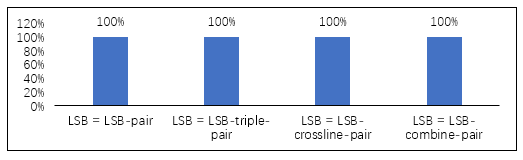
\includegraphics[width=\columnwidth]{image/PSNR.PNG}
\caption{PSNR result}
\label{fig:figure}
\end{figure} 


FIG 4.5  shows the experiment result for using Hae. This approach calculates the gray level difference between original image and watermarked image. If the Hae value difference is lower than 0, it means the distortion is reduced. In this histogram, better means the first embedding method has better distortion reducing performance than the second method. In other word, the better in the histogram represents Haefirst method – Haesecond method < 0.

Comparing application of original LSB replacement with others, an average of 6\% of the images have better distortion reduction than other four LSB-pair methods. LSB-pair takes the lowest at 5.18\%, and LSB-combine-pair is the highest at 6.96\%. As for better Hae value comparing with original LSB replacement, LSB-pair performs worst. Original LSB replacement has 24.53\% of images having higher distortion than using LSB-pair. In contrast, LSB-combine-pair performs the best -- 31.28\% have lower distortion than applying original LSB replacement method. However, the most number of image sets have the same distortion, they occupy about 60-70\%. 

As for comparison of LSB-pair and its variations methods using Hae measurement approach, the result generally looks the same -- about 70\% images have the same Hae value. Nonetheless, when looking at this result in more detail, the features of each method are different. Extension LSB-pair methods (LSB-crossline-pair, LSB-triple-pair, LSB-combine-pair) all have a higher percentage of reducing distortion rather than increasing distortion compared with regular LSB replacement. LSB-crossline-pair performs better than LSB-triple-pair: 18.03\% of images have lower distortion than applying LSB-triple-pair and 9.96\% images have higher distortion, and the rest have the same distortion. 
From this data, we can draw a conclusion that, in most cases, LSB-crossline-pair and LSB-triple-pair have similar performances. In the remaining situations, two thirds of images have less distortion change than applying LSB-crossline-pair. Hence, we can conclude that, the LSB-crossline-pair method have better performance than LSB-triple-pair on Hae measurement approach. In LSB-combine-pair, this is the main reason that crossline pair detection has higher priority than jump pixel detection. As for LSB-combine-pair, it performs better than any other methods.

Table 4.2 shows the summary of Hae. It indicates that Hae of original LSB replacement is 0.0224\%, 0.0642\%, 0.0504\%, 0.0834\% higher than LSB-pair, LSB-crossline-pair, LSB-triple-pair, LSB-combine-pair respectively on average. One interesting thing to note is the maximum of Hae is equal across all methods. Tracing back, we find that the image which cause these outlier values is the same one. In this image, it has three unusual features: over 70\% pixels are in the same colour (gray level: 0); pixel gray level changes sharply; there few LSB pairs which can be detected. With the above findings, we can draw a conclusion: a carrier image with complex compositions, variety of colours (gray levels) and no sharp edges in the image is ideal for applying the LSB-pair methods.

\begin{figure}[h]
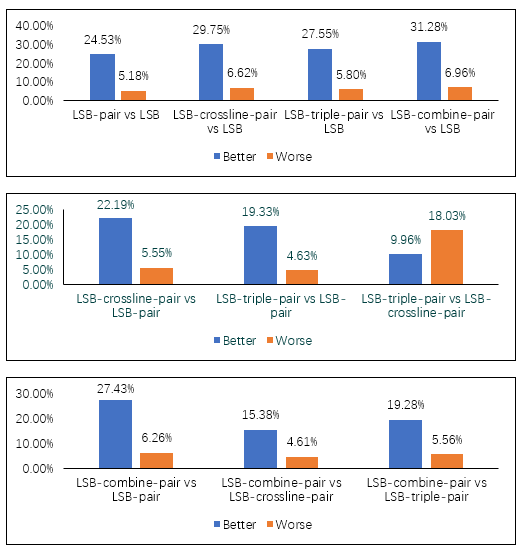
\includegraphics[width=\columnwidth]{image/Hae.PNG}
\caption{Hae result}
\label{fig:figure}
\end{figure} 


\begin{table*}
\centering
\begin{tabular}{|c|c|c|c|c|c|c|}
 \hline
 \multicolumn{7}{|c|}{Histogram absolute error} \\
 \hline
 LSB methods        &Minimum&1st Quartile	&Median	&Mean	    &3rd Quartile	&Maximum\\
 \hline
 LSB&               16950	&42280	        &42868	&43693.44	&43534	        &110376\\
 \hline
 LSB-pair	        &16722	&42274	        &42862	&43683.64	&43526	        &110376\\
 \hline
 LSB-crossline-pair	&16398	&42262	        &42855	&43665.42	&43512	        &110376\\
 \hline
 LSB-triple-pair	&16428	&42268	        &42858	&43671.42	&43518	        &110376\\
 \hline
 LSB-combine-pair	&15832	&42254	        &42851	&43657.03	&43506	        &110376\\
 \hline
\end{tabular}
 \caption{Summary of Hae}
\end{table*}


FIG 12 and table 4.3 indicate the values of using SSIM. Due to the original SSIM value difference is tiny and it is hard for our observation. We use a formula \((1 - SSIM) * 10000\) to zoom in these data. Due to higher SSIM value represents more similar to the original image, in this case, the lower value displayed in the table means the better performance in SSIM. In general, all these extension LSB-pair methods have poorer performance than original LSB replacement. Besides original LSB replacement methods, LSB-triple-pair has the best performance, where 17.19\% of the watermarked images are better than which applying original LSB-replacement; for LSB-pair, this rate is 10.78; 9.81\% for LSB-crossline-pair and 11.56\% for LSB-combine-pair. When comparing LSB-triple-pair with LSB-crossline-pair and LSB-combine-pair, 64.94\% and 89.96\% of images have better SSIM value respectively. 

One thing to note is that LSB-triple-pair has better performance than LSB-pair when compared with original LSB replacement. However, LSB-triple-pair only has 25.55\% of images having better SSIM value than LSB-pair. It means that, if one image applied with LSB-pair method has worse performance than original LSB replacement, it is highly probable that for the same image, LSB-triple-pair may have worse performance than LSB-pair. It also means that for this image, it is very likely that applying LSB-triple-pair yields worse performance than original LSB replacement, and vice versa. As for LSB-combine-pair, it performs the worst in SSIM evaluation; the rates of worse performance are all higher than the rates of better when compared with other methods. However, it does not necessarily mean that LSB-combine-pair is not a suitable digital watermarking embedding method and not friendly to human visual system. Table 4.3 points out that all methods have very narrow gaps with each other, even when the differences have been zoom in ten thousand times. 

\begin{figure}[h]
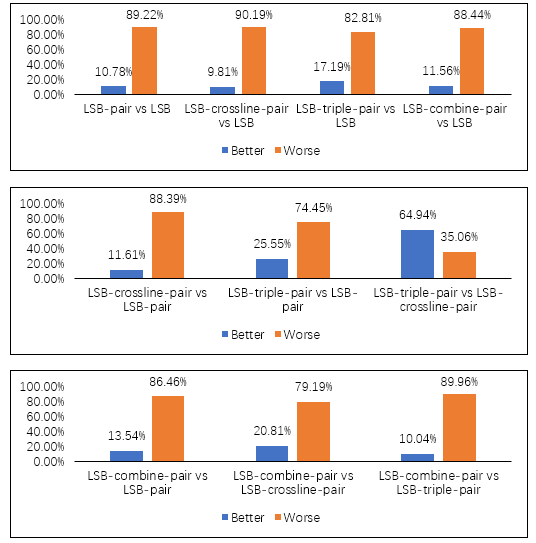
\includegraphics[width=\columnwidth]{image/SSIM.PNG}
\caption{SSIM result}
\label{fig:figure}
\end{figure} 


\begin{table*}
\centering
\begin{tabular}{ |c|c|c|c|c|c|c|  }
 \hline
 \multicolumn{7}{|c|}{(1 - SSIM) * 10000} \\
 \hline
 LSB methods    &Minimum&1st Quartile	&Median	&Mean	&3rd Quartile	        &Maximum\\
 \hline
 LSB	            &2.2705	&20.8321	&27.4459	    &28.8292	&33.5760	&439.2084\\
 \hline
 LSB-pair	        &2.2702	&20.8382	&27.4670	    &28.8401	&33.5981	&439.1730\\
 \hline
 LSB-crossline-pair	&2.2701 &20.8792	&27.5242	    &28.8748	&33.6363	&439.1106\\
 \hline
 LSB-triple-pair	&2.2703	&20.8726	&27.5267	    &28.8617	&33.6324	&438.9516\\
 \hline
 LSB-combine-pair	&2.2700	&20.9028	&27.5861	    &28.8962	&33.6887	&438.9165\\
 \hline
\end{tabular}
 \caption{Summary of SSIM}
\end{table*}


In theory, LSB-crossline-pair has less chances to find pairs than LSB-triple-pair. Because in a \(n \times m\) image, except last two pixels, LSB-triple-pair has \(n \times m -2\) chances of finding a pair. However, LSB-crossline-pair only has \(n \times m - n\) chances, except the pixels that are in the last row. Therefore, if an image is large enough, the method LSB-triple-pair should perform \(1/m\) better than LSB-crossline-pair, because, in theory, it has 1/m more attempts to find pairs. However, the experiment results show that LSB-crossline-pair has better performance in Hae which is against our assumption. 

We suppose this difference is owing to the distance of pixel pair. In FIG 4.7, assuming current pixel is \(P_{7}\), LSB-pair compares it with \(P_{8}\) which has an Euclidean distance of 1; LSB-crossline-pair compares with \(P_{8}\) and \(P_{12}\) which also has Euclidean distance of 1; LSB-triple-pair compares with \(P_{8}\) and \(P_{9}\) with distance of either 1 or 2. Assuming LSB-crossline-pair has better performance in reducing distortion then LSB-triple-pair, we can make a prediction that the lower Euclidean distance will have better performance in LSB-pair extension methods. Therefore, we can predict that LSB-diagonal-pair (\(P_{7}\) with \(P_{8}\) and \(P_{13}\)) has better performance than LSB-crossDoubleLine-pair (\(P_{7}\) with \(P_{8}\) and \(P_{17}\)). However, the additional experiment shows that LSB-crossDoubleLine-pair yields better performance than LSB-diagonal-pair (FIG 4.8 and FIG 4.9). Hence, our previous assumption is invalid. 

In general, there are two shortcomings for the LSB-pair methods: lack of the global view, and pair detection is incomplete for extension methods. In our design, these methods can ensure that the distortion will not increase in each logic iteration when a pixel pair has been found. The fact is, in each logic iteration, the distortion does not increase; however, the Hae experiment results show that there still exist a fair number of distortion increases. This is because these methods do not have an overview of total gray level distribution. For each pixel swapping, distortion can be reduced in this specific logic iteration. Nevertheless, for the whole watermarked image, this iteration of pixel swapping might lead to increase in the total distortion. Another weakness is that the extension methods are incomplete. For example, in LSB-triple-pair, we only find pixel pair between first pixel with second, and first with third. We missed the possibility that the second and the third pixel can make a pair. This is one of the reasons that may explain why LSB-crossLine-pair has better performance than LSB-triple-pair. 


There are no precise rules for selecting which measurement approaches is ideal when the evaluation of image quality is required. The aim of using these approaches is to visualise the distortion changes, which is hard to find out and comparing. PSNR is a measurement which focuses on finding the image energy change for each pixel changes respectively. SSIM is a measurement which is interested in the image structure changes. The Hae is an approach for summing up image pixel gray level distortion. Therefore, from the emphasis of each approaches, the result of Hae is considered as the highest priority in our evaluation. As for PSNR and SSIM, they are considered as assisting evaluation approaches. Their results also need to be pay attention to because they can help to guarantee image quality in an acceptable field after embedding security messages. 

In summary, the performance of distortion reduction sorted from best to worst: LSB-combine-pair>LSB-crossDoubleLine-pair>LSB-diagonal-pair>LSB-crossLine-pair>LSB-triple-pair>LSB-pair.


\begin{figure}[h]
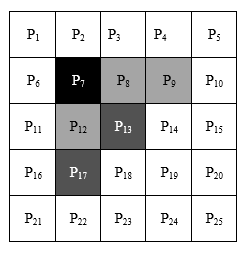
\includegraphics[width=\columnwidth]{image/Euclidean_distance.PNG}
\caption{Euclidean distance}
\label{fig:figure}
\end{figure} 

\begin{figure}[h]
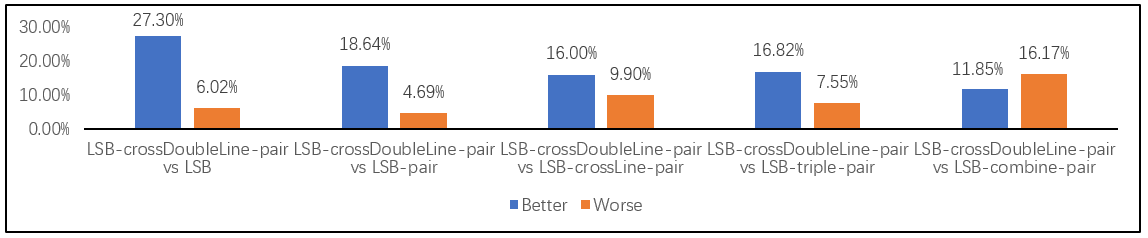
\includegraphics[width=\columnwidth]{image/LSB-crossDoubleLine-pair.PNG}
\caption{Hea for LSB-crossDoubleLine-pair}
\label{fig:figure}
\end{figure} 

\begin{figure}[h]
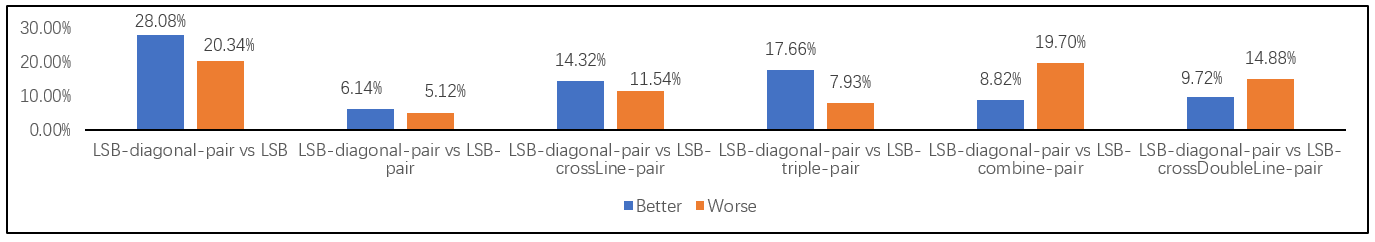
\includegraphics[width=\columnwidth]{image/LSB-diagonal-pair.PNG}
\caption{Hea for LSB-diagonal-pair}
\label{fig:figure}
\end{figure} 

%*******************************************************************************
%****************************** Fifth Chapter *********************************
%*******************************************************************************

\chapter{Conclusion and Future Work}

\ifpdf
    \graphicspath{image/}
\fi



%\section{\label{sec:level1}Conclusion and Future Work}

This thesis proposes a new LSB replacement method called LSB-pair to increase the security of hiding information in digital watermarking technique. This method can reduce watermarked image distortion by finding pixel pairs and swap their values to improve the security of watermarked information. The experiment results show that compared with the original LSB replacement method, LSB-pair can reduce watermarked image distortion but in a very little improvement. Therefore, we designed three extension methods which have better distortion reduction by extending the range of the pixel finding. In order to evaluate each method's performance on distortion reduction, our experiment utilised three image quality measurement approaches: Peak signal-to-noise ratio (PSNR), Histogram absolute error (Hae) and Structural similarity index measure (SSIM).  

The three extension LSB-pair methods we have proposed are: LSB-crossLine-pair, LSB-triple-pair and LSB-combine-pair. Compared with original LSB replacement method, all these methods have the same PSNR result, better Hae result and worse SSIM result. For Hae, LSB-crossline-pair have better performance than LSB-triple-pair. Besides, LSB-combine-pair is better than both LSB-crossLine-pair and LSB-triple-pair. From this discovery, we draw a conclusion that we can improve performance on watermarked image distortion by combining multiple LSB-pair methods together. As for SSIM, the original LSB replacement has the best value and LSB-extension is the worst. Although the differences between each method are insignificant, this experiment result hints that we cannot extend the application range or combine multiple LSB-pair methods arbitrarily in order to have better distortion reduction. At the end of our evaluation, we indicated two existing shortcomings of our methods: lack of global view, and incomplete pixel pair detection.

Future work includes fixing two vulnerabilities we had mentioned, and there is a demand to find a balanced point between SSIM performance and distortion reduction when combining various extension of LSB-pair methods to lower distortion. One additional work is that, these methods should be able to embed messages into colour images, where we need to consider three vectors (RGB) for each pixel instead of only one (gray level).




% ********************************** Back Matter *******************************
% Backmatter should be commented out, if you are using appendices after References
%\backmatter

% ********************************** Bibliography ******************************
\begin{spacing}{0.9}

% To use the conventional natbib style referencing
% Bibliography style previews: http://nodonn.tipido.net/bibstyle.php
% Reference styles: http://sites.stat.psu.edu/~surajit/present/bib.htm

\bibliographystyle{apalike}
%\bibliographystyle{plainnat} % use this to have URLs listed in References
\cleardoublepage
\bibliography{References/references} % Path to your References.bib file


% If you would like to use BibLaTeX for your references, pass `custombib' as
% an option in the document class. The location of 'reference.bib' should be
% specified in the preamble.tex file in the custombib section.
% Comment out the lines related to natbib above and uncomment the following line.

%\printbibliography[heading=bibintoc, title={References}]


\end{spacing}

% ********************************** Appendices ********************************

\begin{appendices} % Using appendices environment for more functunality

% % ******************************* Thesis Appendix A ********************************

\chapter{MATLAB Code}

All codes mentioned in this thesis have been uploaded to GitHub. Link: 

\href{https://github.com/boooooommmmmm/Digital_Watermarking-LSB-pair}{https://github.com/boooooommmmmm/Digital\_Watermarking-LSB-pair}
% % ******************************* Thesis Appendix B ********************************

% \chapter{Installing the CUED Class file}

% \LaTeX.cls files can be accessed system-wide when they are placed in the
% <texmf>/tex/latex directory, where <texmf> is the root directory of the user’s \TeX installation. On systems that have a local texmf tree (<texmflocal>), which
% may be named ``texmf-local'' or ``localtexmf'', it may be advisable to install packages in <texmflocal>, rather than <texmf> as the contents of the former, unlike that of the latter, are preserved after the \LaTeX system is reinstalled and/or upgraded.

% It is recommended that the user create a subdirectory <texmf>/tex/latex/CUED for all CUED related \LaTeX class and package files. On some \LaTeX systems, the directory look-up tables will need to be refreshed after making additions or deletions to the system files. For \TeX Live systems this is accomplished via executing ``texhash'' as root. MIK\TeX users can run ``initexmf -u'' to accomplish the same thing.

% Users not willing or able to install the files system-wide can install them in their personal directories, but will then have to provide the path (full or relative) in addition to the filename when referring to them in \LaTeX.



\end{appendices}

% *************************************** Index ********************************
\printthesisindex % If index is present

\end{document}
